\documentclass{article}

% if you need to pass options to natbib, use, e.g.:
% \PassOptionsToPackage{numbers, compress}{natbib}
% before loading nips_2016
%
% to avoid loading the natbib package, add option nonatbib:
% \usepackage[nonatbib]{nips_2016}

\PassOptionsToPackage{numbers,sort&compress}{natbib}
\usepackage[final]{nips_2016} % produce camera-ready copy

\usepackage[utf8]{inputenc} % allow utf-8 input
\usepackage[T1]{fontenc}    % use 8-bit T1 fonts
\usepackage{hyperref}       % hyperlinks
\usepackage{url}            % simple URL typesetting
\usepackage{booktabs}       % professional-quality tables
\usepackage{amsfonts}       % blackboard math symbols
\usepackage{nicefrac}       % compact symbols for 1/2, etc.
\usepackage{microtype}      % microtypography
\usepackage{graphicx}
\usepackage{subcaption}
\usepackage{titlesec}

%This is added to highlight changes in drafts
\usepackage{xcolor}


\title{Predicting Music Genres \& Artist Popularity}

% The \author macro works with any number of authors. There are two
% commands used to separate the names and addresses of multiple
% authors: \And and \AND.
%
% Using \And between authors leaves it to LaTeX to determine where to
% break the lines. Using \AND forces a line break at that point. So,
% if LaTeX puts 3 of 4 authors names on the first line, and the last
% on the second line, try using \AND instead of \And before the third
% author name.

\author{
  s2759901\\
  %% examples of more authors
  \And
  s2751148\\
 \And
  s2110373\\
  \And
  s2708583\\
}

\begin{document}

\maketitle

\begin{abstract}
 This report explores genre classification and artist popularity prediction tasks within the music industry. Using a Spotify dataset enriched with genre and artist data, we investigate feature transformations and machine learning models to address these tasks. For genre classification, CatBoost achieved the best performance with a weighted F1-score of 0.85, highlighting the significance of categorical features. For artist popularity prediction, Random Forest achieved the best results, with accuracies up to 47\%. Dimensionality reduction and feature importance analysis offered insights into the key attributes driving model decisions. The findings emphasize the challenges of imbalanced datasets and propose future directions, including data augmentation and advanced modelling techniques, to enhance classification performance and interpretability.

\end{abstract}

\section{Introduction}

In an age of unprecedented content consumption, identifying audience preferences has transformed from a trivial task into a sophisticated data-driven effort. Trends in music reveal much about cultural tastes, social currents, and even the shared mood of a population. A platform that not only knows people's favourite genres, songs, or artists but also anticipates emerging trends, can predict and adapt their offers and recommendations in the future. This is the essence of genre classification and popularity prediction: to categorize content and forecast the future trajectory of its popularity.

\subsection{Description of the task}

Drawing on Spotify's \textit{`Top 200'} songs playlists, our project aims to offer significant insights into music trends. This project will address two principal objectives to understand both the stylistic elements of
music and the factors driving artist popularity, each linked with a research question:

\textbf{Genre Classification:} Our first task focuses on identifying the features that are most indicative of a song's genre. By applying machine learning algorithms, we aim to accurately classify songs into specific genres like pop, classical, or rock, amongst 12 other genres. This task aims to dissect qualitative and acoustic characteristics metadata to pinpoint the essence that distinguishes one genre from another, that is, \textbf{``What indicators are most helpful for discovering the genre of a song?"}

\textbf{Artist Popularity Prediction:} Understanding and predicting the popularity of music artists involves analysing various factors, such as an artist's musical characteristics, collaboration patterns, and career trajectories. The goal is to classify artists into three popularity categories (\textit{High}, \textit{Medium}, \textit{Low}) and assess the effectiveness of various machine learning models for this task. By addressing the question, \textbf{``Can an artist's popularity be predicted?"}, this project aims to contribute to a deeper understanding of the music industry's dynamics.
Tasks (Appendix~\ref{appendix:hit_song} and Appendix~\ref{appendix:temporal_genre_prediction}) were considered for this task, However, in order to make use of the whole dataset, \textbf{Artist Popularity Prediction} was chosen so that some temporal features were used.
  
\subsection{Relevant background and related previous work}

Genre classification is a well-researched area in music information retrieval. Various machine-learning approaches have been applied to genre classification, leveraging multiple types of data, such as lyrics, audio previews, and album artwork \cite{dammann2017genre}, to enhance predictive accuracy. Techniques like Naive Bayes, Recurrent Neural Networks, and k-Nearest Neighbors have shown that combining diverse inputs can capture distinct genre characteristics and improve classification performance \cite{werner2020organizing}. However, other methods limit the scope to using audio features like danceability and tempo to predict genres, although these approaches often face challenges due to genre overlap, showing the complexity of music classification \cite{hendri2024comparation}. These studies highlight the complexity of the task, offering an analysis of the features normally used in genre classification, techniques, and most effective models in the task, together with the difficulties encountered. This provides a strong foundation for our project’s goal.

Beyond genre classification, previous studies \cite{Mining_and_Forecasting_Career_Trajectories, Collaboration_Profiles_Impact} have explored the dynamic factors that influence an artist's success. This task extends these ideas by aggregating artist-level data from Spotify, including musical characteristics (e.g., danceability, energy, loudness) and longevity. 
Taken together, these studies provide the foundation for understanding and forecasting music trends.

\subsection{Relevance of the task}

Achieving an accurate classification of genres and predicting artist popularity holds substantial value for current services like Spotify. This dual focus helps enhance the user experience by tailoring music discovery to individual tastes and aids in strategic content management. By understanding the dynamics behind music genres and predicting an artist's success, this project positions itself as a critical tool for navigating the complexities of the music industry. It aims to provide deeper insights into how societal trends and cultural influences impact musical preferences, offering valuable data for both industry and academic research.

\section{Data Preparation}

For the first task, several datasets are needed. Starting from the original \textit{``Top 200 playlists"} Spotify dataset, ranging from 01/01/2017 to 31/05/2023, we incorporate two additional datasets, as the genre of a song is indispensable for genre classification. This initial dataset does not provide any information related to this label, however, it contains the samples and features used for classification purposes, which are used exclusively in our second task.

The first additional dataset consists of two specific columns: the title of each song and its respective genre. This information was extracted using the Spotify API, which provides comprehensive details on a wide array of musical tracks, including the ones on this project. For the purposes of our study, we selectively gathered only these two pieces of data from the available information, successfully relating each song with its genre, resulting in a total of 415 unique genres.
This vast number of classes can dilute the dataset, leading to insufficient data for each class and greatly increasing model complexity, which hinders the model's ability to generalize and affects the project's overall outcome. To address this challenge, we reduced the classes by grouping these genres into a broader category, creating a \textit{``Parent Genre"} column.  

To assign the parent genres, we scrape the web page \cite{ParentGenreSite}, which provides expert knowledge on broader music genres. Parsing the HTML using BeautifulSoup library in Python, and extracting the values for the Parent Genre class we are left with the set of following genres: \textit{('latin', 'pop', 'R\&B', 'Hip Hop', 'country', 'rock', 'Electronic', 'World/Traditional', 'Folk/Acoustic', 'metal', 'easy listening', 'blues', 'classical', 'jazz')}. 

This finalized dataset enables us to advance with the tasks at hand. Nonetheless, it is imperative to conduct an initial exploratory data analysis of this dataset to ensure its adequacy for the intended applications.

\section{Exploratory Data Analysis}


The dataset contains diverse information of 8,684 unique songs across 14 genres and 2,794 artists, spread over 2,336 dates. Features consist of continuous variables representing musical aspects of a song, including Danceability and Energy, and categorical fields like Continent and Nationality, limited to a few unique values. We split our dataset into training and hold-out test sets with an 80 to 20 ratio respectively. It is worth noting that this ratio will not be exactly preserved, as first, all the instances of a song will be compacted in one row. After the split, we will again expand it to the original number of samples, to avoid any data leaking \cite{Test_Training_Leakage} from the train to the test set.

It is convenient to analyse the distribution of track genres (see Figure~\ref{fig:genre_distribution}). This plot provides a clearer and more concise view of genre representation and shows a high imbalance in genre distribution, which may influence the techniques applied in machine learning modelling, as well as the results or metrics of subsequent analyses.

Several preprocessing steps were necessary during the exploratory data analysis in our training set.
To handle outliers in the data, we applied the Interquartile Range (IQR) method \cite{lane2003introduction}. This approach helps mitigate the influence of extreme values, enhancing the robustness of the analysis.

Additionally, to reduce computational complexity, some categorical features were simplified. 
Apart from the genre feature, some feature distributions were highly unbalanced, with the majority of occurrences concentrated in just a few values. For instance, in the \textit{Nationality} feature we retained the 15 most common nationalities and grouped all others under a 16th category, ``Others.'' Also, additional columns were created from the \textit{Date} feature for analysis and convenience, including \textit{Month Quarter} (split as 1 for days 1-15, and 2 for days 16-31), \textit{Month}, and \textit{Year}.
The \textit{Instrumentalness} feature was replaced by a binary variable, \textit{Is\_Instrumental}, due to its distribution being heavily concentrated near zero (as seen in Figure~\ref{fig:preprocessing_comparison}). This transformation simplifies the feature, distinguishing between instrumental and non-instrumental tracks more effectively.

To prepare the data for analysis, we applied different normalization techniques based on the distribution of each feature (See Figure\ref{fig:preprocessing_comparison}):
\textbf{Standardization}: This process was used for features with approximately normal distributions, such as \textit{Rank}, \textit{Danceability}, \textit{Energy}, \textit{Valence}, \textit{Points (Total)}, and \textit{Points (Ind for each Artist/Nat)} \cite{standardization_source}.
 \textbf{Log transformation}: This was applied to features with skewed distributions, including \textit{Loudness}, \textit{Speechiness}, \textit{Acousticness}, and \textit{Instrumentalness} \cite{log_transformation_source}.
\begin{figure}[h]
    \centering
    % First figure (Before preprocessing)
    \begin{subfigure}[b]{0.45\textwidth}
        \centering
        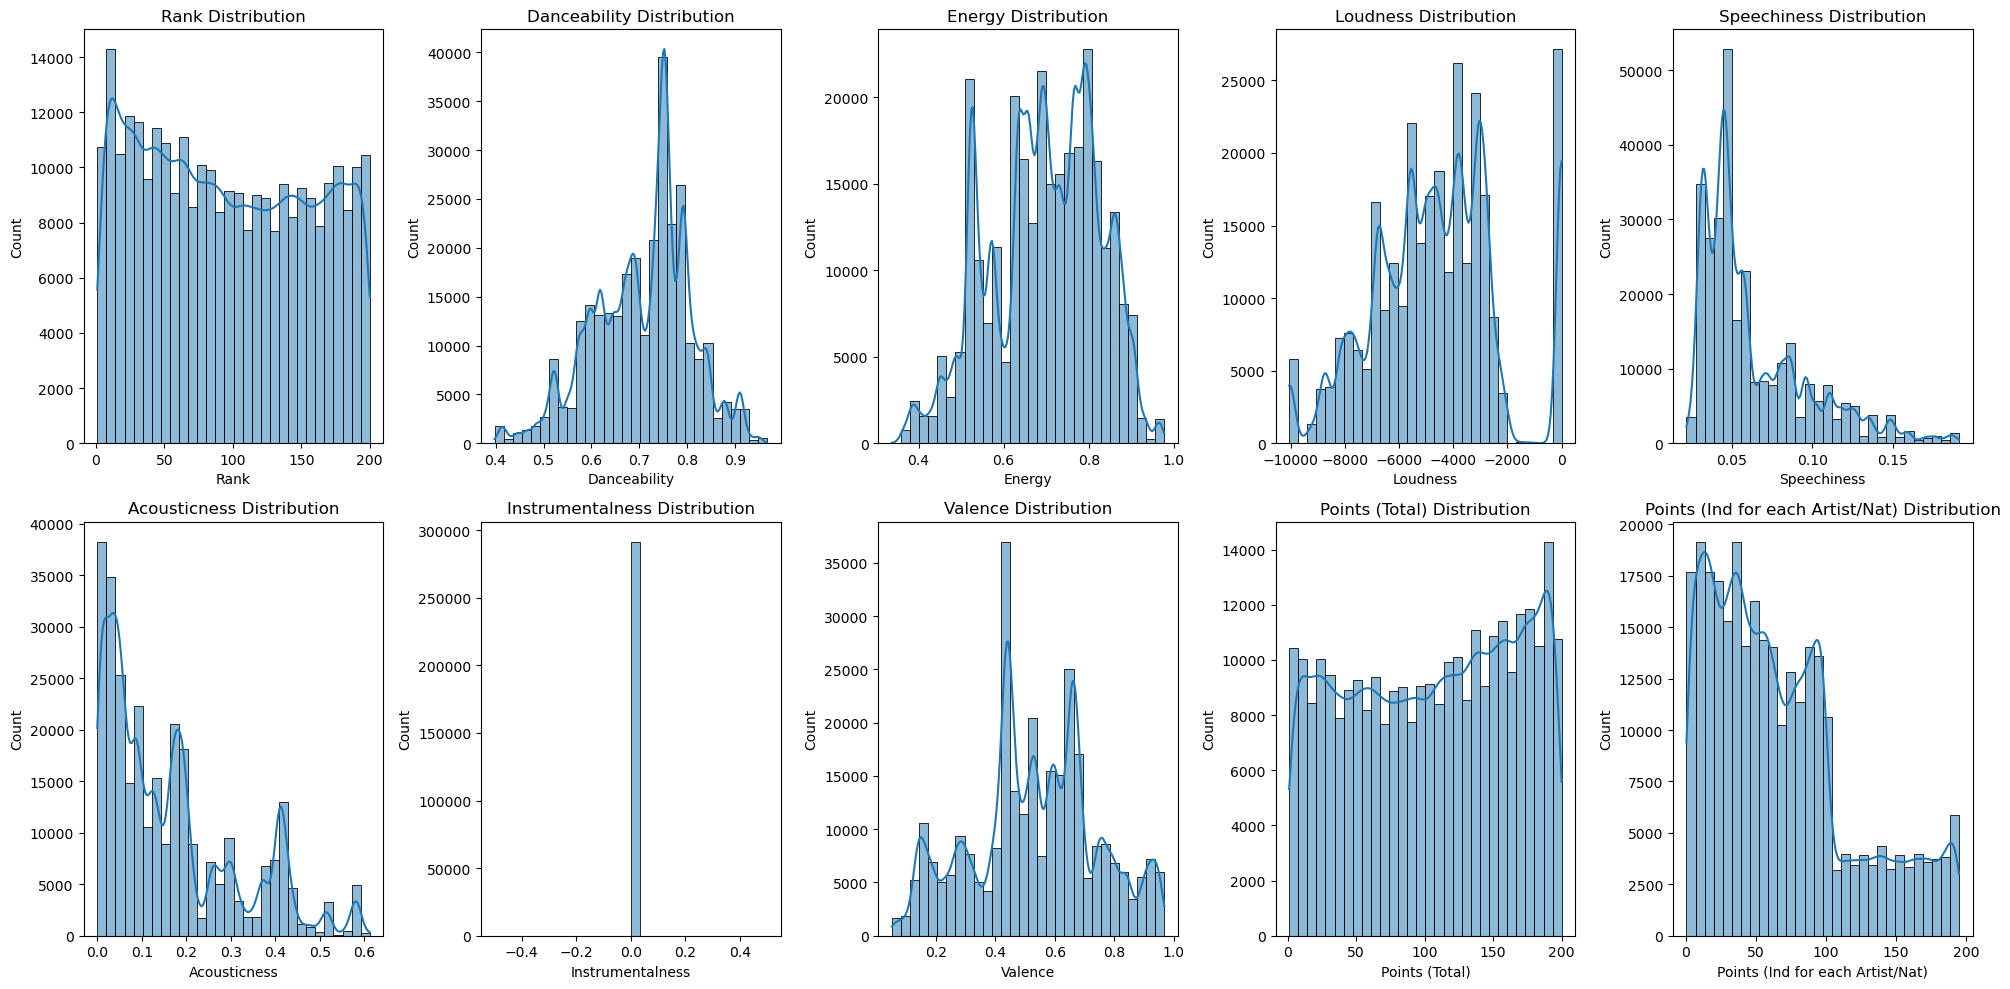
\includegraphics[width=\textwidth]{data_before_preprocessing.png}
        \caption{Distribution of features before preprocessing}
        \label{fig:before_preprocessing}
    \end{subfigure}
    \hfill
    % Second figure (After preprocessing)
    \begin{subfigure}[b]{0.45\textwidth}
        \centering
        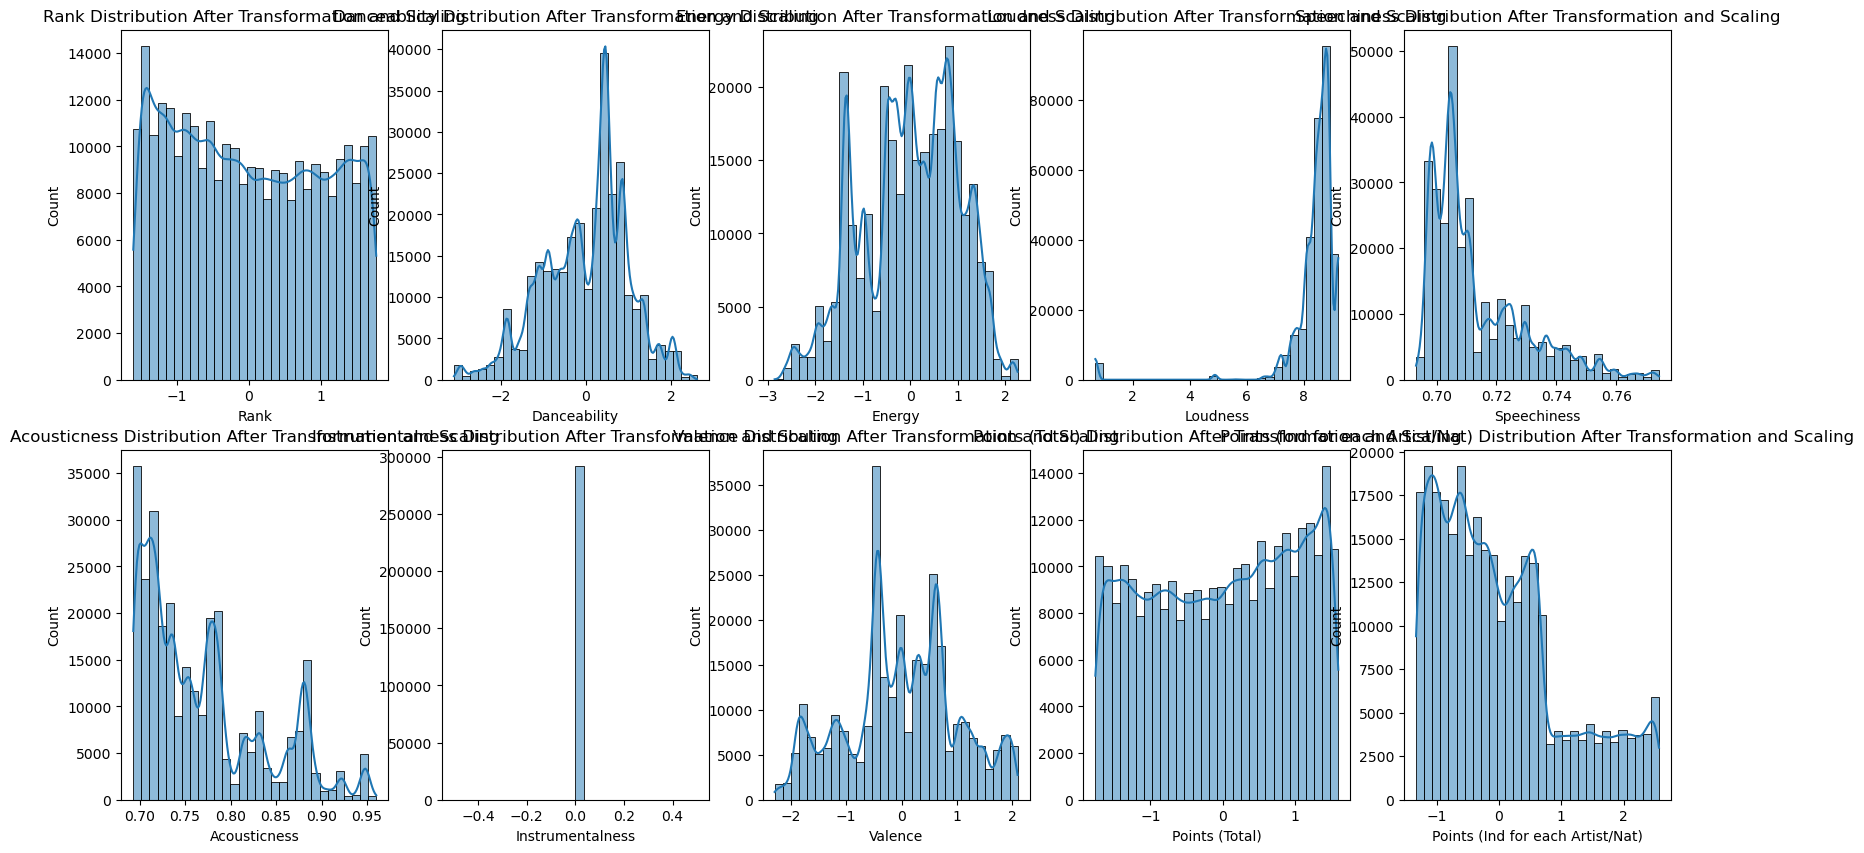
\includegraphics[width=\textwidth]{data_after_preprocessing.png}
        \caption{Distribution of features after preprocessing}
        \label{fig:after_preprocessing}
    \end{subfigure}
    \caption{Comparison of feature distributions before and after preprocessing}
    \label{fig:preprocessing_comparison}
\end{figure}

A correlation matrix was computed to identify relationships between numerical features in the dataset. To avoid multicollinearity and reduce redundancy, features with an absolute correlation above 70\% \cite{shrestha2020detecting} were removed. The \textit{Points (Ind for each Artist/Nat)} and \textit{Points (Total)} features were removed.


Moreover, we employed PCA, t-SNE, and UMAP for the visualization of the dataset, revealing a complex dataset with no clear linear separability or distinguishable clusters, as detailed in Figure \ref{fig:dimensionality_reduction}. A comprehensive analysis of these findings is presented in Appendix~\ref{appendix:dim_red}.


\section{Task 1 - Genre Prediction}

This task aims to create a classifier that correctly predicts the genre of a song based on its features. Thus, several models are tested for this purpose. With that, the importance of the features are extracted from a trained model in the task. 

Besides quantitative features that measure musical aspects of a song, such as 'valence' or 'energy', categorical features are also employed. This category comprises features like artist names or their corresponding country of origin. Cultural style differences between nations and the predominance of certain singers in a field might be indicative of the genre of song, contributing to the classification. 

\subsection{ Classification algorithms
} \label{sec:Classification algorithms1}

We compare four learning algorithms to evaluate performance of specialized boosting algorithms against more general-purpose methods. Due to the difference in their nature, we compare four well-known models: Logistic Regression (LR) as a simple interpretable baseline, Random Forest (RF), Gradient Boosting Classifier (GBC) ensemble learning techniques that handle complex, non-linear patterns and Categorical Boosting (CatBoost) which is specifically designed for categorical features.

\textbf{Random Forest} is a powerful ensemble learning technique that combines multiple decision trees to make predictions\cite{Breiman2001}. Each tree in the forest is trained on a random subset of data and features, reducing overfitting and improving the model's generalization ability. This diversity in the trees leads to more accurate and robust predictions. \textbf{Logistic regression} is a statistical model that is particularly useful for binary classification problems\cite{Hosmer2013}. The model fits a logistic curve to the data, mapping input features to a probability between 0 and 1. Despite its simplicity, it is widely used due to its interpretability and efficiency. \textbf{Gradient boosting classifier} is an ensemble learning technique that sequentially builds decision trees, with each tree correcting the errors of the previous ones\cite{Friedman2001}. It uses gradient descent to minimize the loss function, iteratively improving the model's accuracy. It is known for its powerful performance and often outperforms other models, especially when dealing with complex patterns in the data. \textbf{Categorical Boosting} is a gradient boosting algorithm designed to handle both numerical and categorical features efficiently. Unlike traditional boosting algorithms, CatBoost natively processes categorical features without requiring explicit encoding, leveraging a novel target-based encoding method while mitigating the risk of data leakage. It employs Ordered Boosting to address overfitting and relies on symmetric decision trees for faster training and inference. It is highly effective for imbalanced datasets, and is robust across various domains \cite{prokhorenkova2018catboost}.

\subsection{Methods}

Adding to the preprocessing steps in EDA for this task, we remove the duplicates of songs with same 'id' and further process the categorical features of the data such as 'Nationality' and 'Artists' in order to get some numerical values for the model to train on. We tried 2 different encoding techniques for this purpose; Label encoding and feature hashing. Label encoding is a simple technique that assigns a unique integer to each category, which assumes ordinality in the feature. Feature hashing is more complex technique that uses a hash function to map each categorical value to a numerical value within a fixed range. It does not assume ordinality, and it is particularly useful when dealing with high-cardinality categorical variables\cite{weinberger2009feature} which makes it suitable for our case.

All of the models that are mentioned in section~\ref{sec:Classification algorithms1} are trained on the same train data by using stratified 5-fold cross-validation and all the models are tuned for the best hyper-parameter settings in the set range with Gridsearch method. GridSearch and cross-validation are techniques used to optimize and evaluate a model's performance. GridSearch systematically searches for the best combination of hyperparameters (e.g., max depth) by trying all specified parameter combinations, while Stratified K-Fold cross-validation splits the data into multiple folds to ensure the model is trained and validated on different subsets, reducing the risk of overfitting. Together, they ensure the model's hyperparameters are fine-tuned for the best performance and validated robustly on unseen data. Then they are all tested on the same test data with the best set of hyperparameters.

\subsection{Metrics} \label{sec:Metrics1}

As seen in the EDA, the class distribution is highly imbalanced, making accuracy alone an unreliable performance metric that can lead to wrong conclusions. Dominance of majority classes necessitates metrics that assess performance on minority classes. 

The confusion matrix (Appendix ~\ref{appendix:confusion_matrix}) provides a breakdown of true positives, true negatives, false positives, and false negatives for each class. It allows a more nuanced and granular evaluation of predictions, ensuring areas of poor performance are identifiable and addressable. To address imbalance, the weighted F1 score is used as the primary metric. By combining precision and recall and weighting each class proportionally, the weighted F1 score ensures balanced evaluation. This approach prioritizes identifying minority class instances and minimizing false positives, offering a comprehensive and fair assessment while reducing risks of critical errors in minority predictions.

\subsection{Results}

Table~\ref{tab:performance} shows that CatBoost beat all other models, with an accuracy of 0.86 and a weighted F1-score of 0.85. Among the studied algorithms, RF and GBC performed well but fell behind CatBoost in terms of categorical feature handling. LR, which served as the baseline, performed poorly, particularly under the label encoding setting, with an accuracy of 0.41 and a weighted F1-score of 0.42.

When comparing encoding strategies, feature hashing consistently outperformed label encoding across all models, demonstrating its usefulness for high-cardinality categorical data such as artist names and nationalities. CatBoost, on the other hand, achieved its peak performance without the need for explicit categorical feature encoding, thanks to its built-in handling of such data.

We further examined the results by looking at the features importances of selected models (RF and CatBoost) in order to find the most helpful features for classification, as it was one of our main motivations.  Feature importance analysis found that numerical features including \textbf{danceability, valence, and acousticness} were important for genre classification across models. However, CatBoost prioritized categorical data such as \textbf{artists and countries}, demonstrating its ability to efficiently capture high-cardinality feature relationships. In contrast, Random Forest’s impurity-based feature importance spread significance more uniformly across numerical features, indicating less confidence in the utility of categorical variables. Since many artists predominantly produce music in specific genres(e.g. Metallica is linked to rock and metal) and musical styles often vary significantly by country(e.g. Reggaeton is predominantly associated with Latin America) or region due to cultural preferences the feature importance of CatBoost aligns well with our hypothesis.

Despite these gains, the confusion matrix ~\ref{fig:confusion_matrix} revealed persistent issues with underrepresented genres. CatBoost performed well in majority categories such as ``pop'' and ``rock,'' but had lower recall in minority genres such as ``jazz'' and ``classical.'' This imbalance indicates the need for further efforts to improve minority genre classification, such as oversampling or advanced cost-sensitive learning \cite{krishnapuram2011cost}.


\begin{table}[h!]
\centering
\captionsetup{belowskip=12pt,aboveskip=8pt} 
\begin{tabular}{|c|c|c|c|c|}
\hline
\textbf{Algorithm} & \textbf{Encoding Type} & \textbf{Accuracy} & \textbf{Weighted F1 Score} \\
\hline
RF  & Feature Hashing & 0.77 & 0.75 \\
GBC & Feature Hashing & 0.73 & 0.73 \\
LR  & Feature Hashing & 0.69 & 0.68 \\
\hline
RF  & Label Encoding  & 0.51 & 0.45 \\
GBC & Label Encoding  & 0.45 & 0.41 \\
LR  & Label Encoding  & 0.41 & 0.42 \\
\hline
CatBoost & -  & \textbf{0.86} & \textbf{0.85} \\
\hline
\end{tabular}
\caption{Model Performance under Different Categorical Encoding Settings}
\label{tab:performance}
\end{table}



\section{Task 2 - Artist Popularity Prediction}

The aim is to identify key factors that allow us to categorize an artist's popularity into three distinct popularity categories: High, Medium, and Low by analysing a combination of musical attributes, collaboration patterns, and career trajectories. 

\subsection{Classification algorithms}

We implemented \textbf{XGBoost} \cite{Friedman2001}, \textbf{SVC} \cite{Brereton2010Support}, and \textbf{Random Forest} \cite{Breiman2001}, as a result of their ability to handle complex, high-dimensional data. These models were chosen based on their demonstrated success in non-linear tabular data (refer to PCA in the Appendix~\ref{appendix:pca_non_linear_data}).

\subsection{Methods}
Additionally, for this task, we aggregate track-level data from Spotify at the artist level, engineering several features to support classification. Acoustic features include the average values for Danceability, Energy, Loudness, Speechiness, Acousticness, and Valence, capturing an artist's overall musical style. 
Temporal features include the most recent year of release (\texttt{most\_recent\_year}) and the range of active years (\texttt{active\_years\_range}), indicating career longevity. Popularity metrics include the mean rank of an artist's tracks on Spotify charts (\texttt{mean\_rank}) and a secondary rank-based feature (\texttt{target\_mean\_rank}). To simplify the task, artists are grouped into three popularity categories (High, Medium, Low) using quantile bins of \texttt{mean\_rank}, ensuring balanced class distributions.
The models were trained using a stratified 80/20 train-validation split to preserve class balance in both sets. Hyperparameters were set after doing a GridSearch.

\subsection{Metrics}
Similar to section~\ref{sec:Metrics1}, we prioritised the \textbf{weighted F1-score} to evaluate model performance, particularly during the grid search for hyperparameter optimization, ensuring a balance between precision and recall across all classes. Additionally, we evaluated \textbf{Accuracy}, which offers a straightforward measure of overall correctness and is well-suited for balanced datasets.

\subsection{Results}

Table~\ref{tab:f1_class_comparison} summarizes the accuracy and F1-scores for each class across the top three performing models after hyperparameter tuning (see Appendix~\ref{appendix:hyperparameter_tuning} for details). Results from some simpler models were also considered (Appendix~\ref{appendix:other_modelling_results}) but are not included in the table.



\begin{table}[h]
\centering
\begin{tabular}{|c|c|c|c|c|}
\hline
\textbf{Model}      & \textbf{Accuracy} & \textbf{F1-Score (High)} & \textbf{F1-Score (Medium)} & \textbf{F1-Score (Low)} \\ \hline
\textbf{SVC}        & 45\%              & \textbf{0.56}            & 0.32                       & 0.43                   \\ \hline
\textbf{XGBoost}    & 45\%     & 0.54                     & 0.26                       & \textbf{0.50}          \\ \hline
\textbf{Random Forest} & \textbf{47\%}           & 0.54                     & \textbf{0.35}              & 0.51                   \\ \hline
\end{tabular}
\captionsetup{belowskip=12pt,aboveskip=8pt}
\caption{Comparison of accuracy and F1-scores for each class across the models on test data.}
\label{tab:f1_class_comparison_tuned}
\end{table}

The lack of significant performance gains with complex models highlights the task's difficulty, showing that \textbf{improved data}, rather than better models, is needed. Modest model performances suggest that artist popularity is influenced by complex, multi-dimensional factors not fully captured in the dataset. Social, cultural, and economic variables likely play a role beyond musical attributes. Popularity is not solely driven by quantitative features (e.g., energy) but also by external elements like marketing, viral trends, or platform biases. Lower F1-scores for the ``Medium'' popularity class reveal challenges in recognizing artists on the margin, suggesting fluid distinctions between popularity levels. In summary, accurately predicting artist popularity with the current dataset is challenging. Future improvements are discussed in Appendix~\ref{appendix:future_work}..

\section{Conclusion}

Our investigation into genre classification using the Spotify dataset presents significant insights. The CatBoost model, specifically designed to handle categorical data, emerged as the superior classifier with an impressive weighted F1 score of 0.85. This model's ability to process high-cardinality features such as artist names and national origins without explicit encoding proved particularly effective, demonstrating its effectiveness in identifying cultural and stylistic nuances inherent in musical genres. Notably, feature hashing outperformed label encoding across all models, affirming its suitability for managing complex categorical data in musical datasets.

In our second task, artist popularity prediction, our results were more mixed, reflecting the complexity of predicting popularity based solely on quantitative and musical features. Despite the deployment of sophisticated machine learning models like XGBoost and Random Forest, the performance indicators remained modest. This task underscored the challenge of capturing the influences on artist popularity, which extend beyond measurable attributes to include social, cultural, and economic factors that are not readily quantifiable. The nuanced performance across different popularity classes further highlighted the variability and transient nature of what defines artist popularity, suggesting that future models might benefit from integrating broader datasets and emphasizing the value of tailored algorithms in domain-specific applications like the dynamic landscape of music popularity.

\bibliography{refs.bib}
\bibliographystyle{plain}

\section{Appendices}

\appendix

\section{Data preparation details}

We already mentioned how we extend our dataset in our Data Preparation section, here we will provide the important details. First by using 'Get Track' functionality of Spotify API we get the corresponding artist id. After obtaining all the unique artist ids we use 'Get Artist' functionality to get the genre information of the corresponding artist. Many of the artist are linked with several genres that are closely related like 'dance-pop', 'pop', 'uk-pop'. Since they all belong to a one bigger parent genre we only get the first genre for each artist and assign it to all their songs in our dataset.

To obtain the parent genre information, we use the website \textit{`https://www.chosic.com/music-genre-finder/'}, which provides details about the parent genres of base genres recognized by Spotify. A Python scraper was developed to automate this process. The scraper sends an HTTP request to the website, appending each base genre to the URL to fetch the corresponding HTML content. This HTML is then parsed using the \textit{BeautifulSoup} library to extract the \textit{parent-genre} information. The process is repeated iteratively for all unique base genres, and the extracted relationships are stored in a CSV file named \textit{parent\_genre.csv}, representing the child-parent genre hierarchy for most genres.

\section{Visualization}
\label{appendix:dim_red}

To complement the exploratory data analysis, three dimensionality reduction methods were applied to the dataset: PCA, t-SNE, and UMAP, in order to visualize the dataset in a lower-dimensional space for better interpretability.

\begin{figure}[ht]
    \centering
    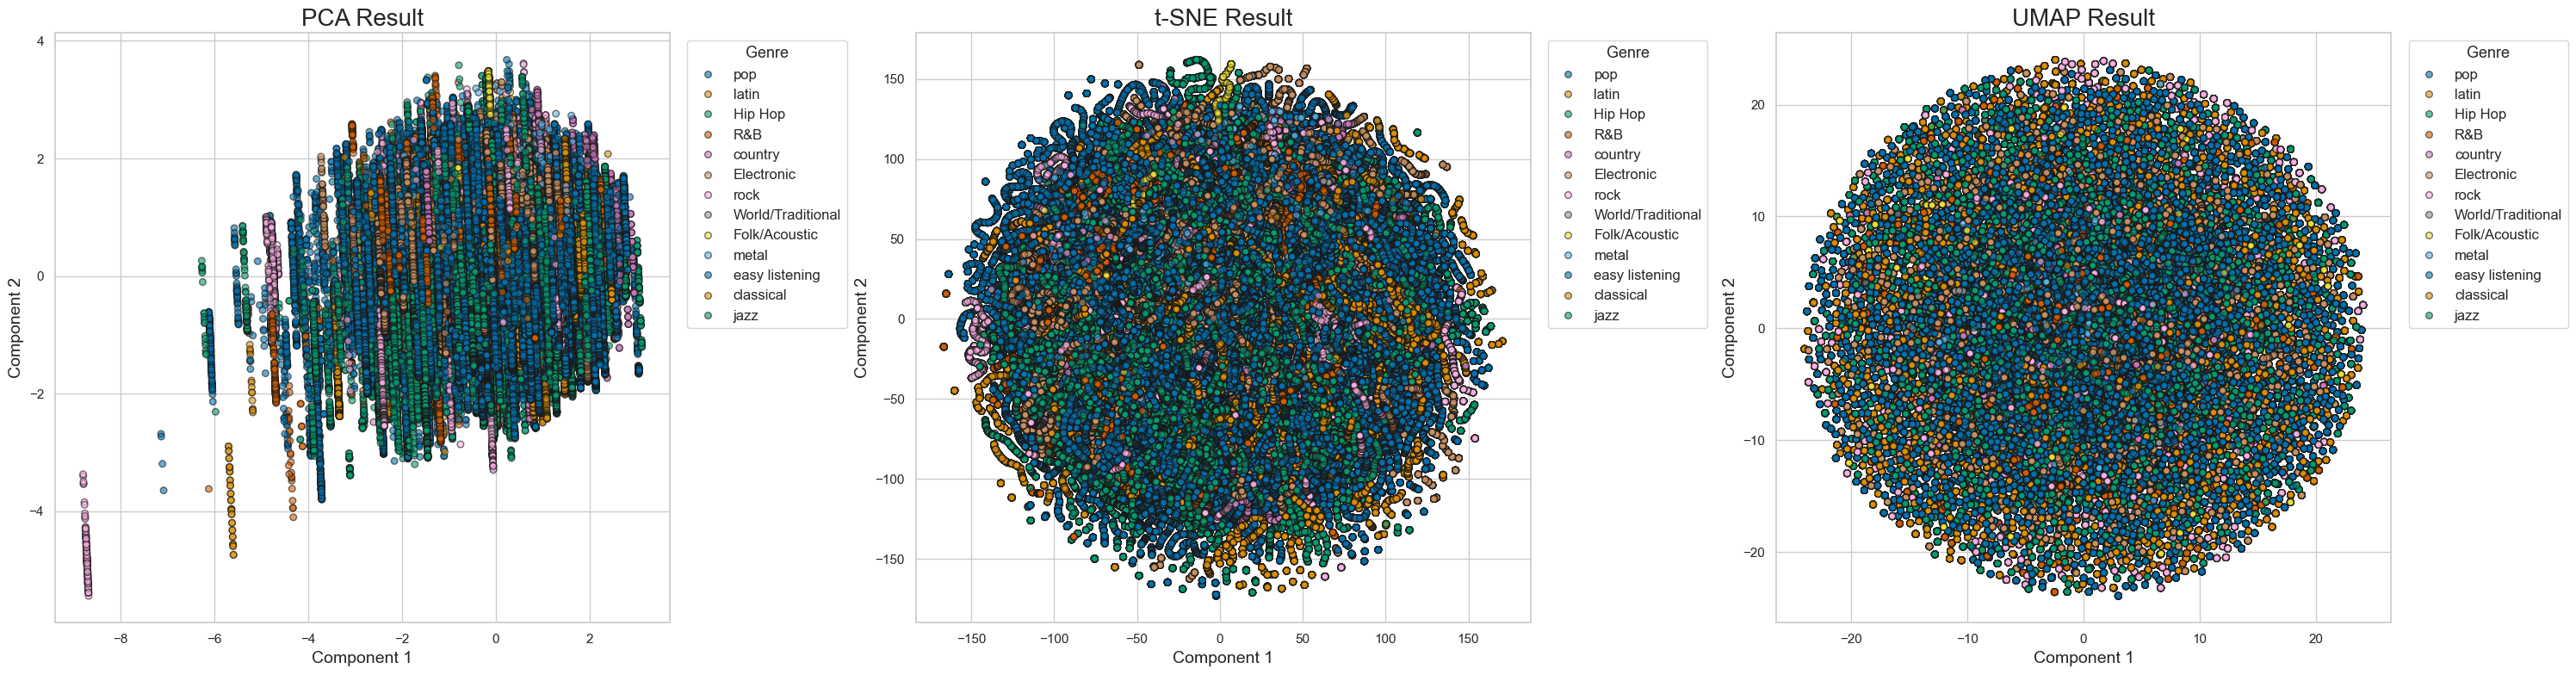
\includegraphics[width=\textwidth]{Dimensionality_Reduction_Comparison.png}
    \caption{Dimensionality reduction comparison: PCA, t-SNE, and UMAP results visualized. Each plot shows data projected onto the first two components of the respective dimensionality reduction technique.}
    \label{fig:dimensionality_reduction}
\end{figure}                

The results, as shown in Figure~\ref{fig:dimensionality_reduction}, indicate that the dataset does not exhibit clear linear separability, as well as the presence of a highly imbalanced distribution of samples per genre. Further analysis in PCA reveals that the first two principal components account for a cumulative variance of only 59.95\%, with diminishing contributions from subsequent components (e.g., Component 3: 19.02\%). The variance across all the 7 numerical variables keeps diminishing, leaving the last 3 components with negligible cumulative explained variance of 4\%. This suggests that the dataset's variance is distributed across, mainly, four dimensions, that is, four features are  responsible for capturing the data's structure using linear projections.
This is an important starting point in our first task, establishing a bound to the number of representative features were looking for.

Non-linear methods like t-SNE and UMAP were also explored to uncover potential patterns or clusters within the data. However, these visualizations also failed to reveal distinct separability between genres, and clusters remained indistinguishable. This outcome might result from the inherent overlap between genres.

These dimensionality reduction methods did not yield clear separable clusters, though the explained variance from PCA provides valuable insight: the dataset has significant complexity, with no initial linear separability. These findings highlight the need of advanced machine learning techniques capable of handling non-linear data distributions in subsequent stages of this project. 

\section{Label reduction}

As noted in the EDA, we manually relabelled songs to their parent genres, a time-consuming and subjective process. To automate this, we propose using Sentence-BERT \cite{Reimers2019} embeddings to cluster sub-genres into parent genres efficiently and scalable. This method leverages the model's ability to capture semantic similarities among genre names (using all-mpnet-base-v2 for its superior performance). After extracting embeddings, PCA is applied to reduce dimensions for efficient clustering, followed by agglomerative clustering, which suits hierarchical structures like genres. The number of clusters is validated using the silhouette score, which evaluates clustering quality based on within-cluster similarity and between-cluster dissimilarity, ranging from -1 (poor) to 1 (good). 

After trying different numbers of clusters we obtained the best silhouette score 0.433 with 3 clusters. It should be noted that the number of clusters is far from the expected range (10-15) which may be the effect of over smoothing in PCA. The distribution of classes could be better seen in ~\ref{fig: 2D Visualization of Clusters with Hierarchical Clustering} In order to get the solidity of our cluster we calculated the adjusted rand index (ARI) between the manually reduced classes and automatically reduced classes. ARI is used to evaluate the similarity between two data clusterings, accounting for chance and it also ranges between -1 and 1 where 1 means high agreement between the clusters. We got 0.365 ARI score which indicates that the clusters are somewhat aligned but not strongly. Then tried these clusters on task 1 
 where we trained a logistic regression(with hashed features) and CatBoost models on the automatically clustered data in order to compare the obtained results. Same hyper-parameter search and validation techniques are applied and we got 0.744 weighted F1 score on the test data for logistic regression and 0.90 for CatBoost model. It is higher than the weighted F1 scores(0.69, 0.86) obtained by our models on the main original data. This suggests that the automatic method likely captures relationships between genres more effectively than the manual approach. If the goal is higher performance and better class separation, the automatic reduction appears to be the better option, though further analysis and potential refinement of the grouping strategies may provide even better results. Mainly because automatic approach lacks semantic meaning. For instance, clustering might group genres like jazz and electronic due to overlapping acoustic features, even though they are distinct in musical taxonomy. A person knowledgeable about music can evaluate whether the clusters make sense from a musical or cultural perspective. For future research, combining these two could be examined where it starts with the automatic clustering as a baseline then a domain expert analyses the clusters and adjusts them based on musical knowledge or cultural relevance.

\begin{figure}[h]
    \centering
    % Adjust the width to reduce the size of the image
    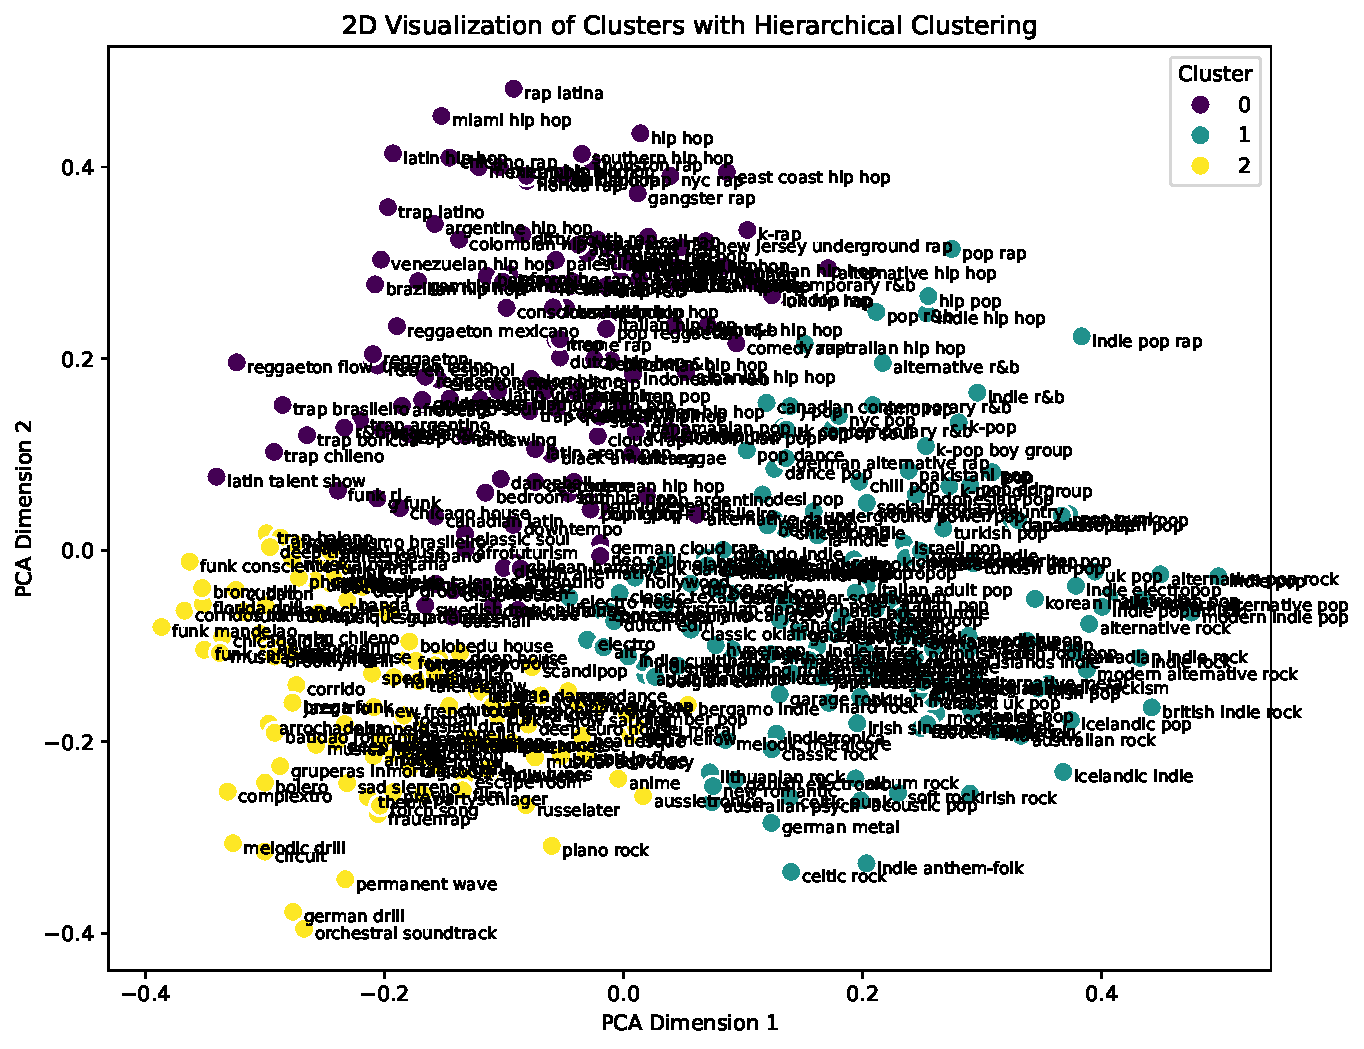
\includegraphics[width=0.7\textwidth]{genre_clusters_auto.pdf}
    \caption{Distribution of genres using word embeddings generated from Sentence-BERT model.}
    \label{fig: 2D Visualization of Clusters with Hierarchical Clustering}
\end{figure}


\section{Future work}
\label{appendix:future_work}

To address the limitations identified, several directions for future work can be considered in task 2:


\textbf{Data Augmentation} can mitigate the limitations of a small dataset, synthetic data generation techniques could be employed, such as GAN-based data augmentation \cite{antoniou2017data}, may help increase the effective size and diversity of the data, enabling models to generalize better.

\textbf Using \textbf{Broader Hyperparameter Tuning} for future work could explore advanced hyperparameter optimization techniques such as Neural Architecture Search (NAS) \cite{zoph2016neural}. These kinds of methods allow for more efficient exploration of hyperparameter spaces and may yield better configurations than the ones explored in this second task.

Aggregating by artist may lose critical temporal patterns. Future work could explore \textbf{time-series models}, such as LSTMs \cite{hochreiter1997long} or Temporal Convolutional Networks (TCNs) \cite{lea2017temporal}, to capture temporal trends in features like \texttt{most\_recent\_year} or \texttt{active\_years\_range}.

\textbf{Larger and More Diverse Datasets:} Expanding the dataset by integrating other sources of music-related data, such as streaming statistics or user-generated playlists, can provide additional diversity and increase the dataset size. Initiatives like the Million Song Dataset \cite{bertin2011million} can be leveraged to supplement the current data.

Employing \textbf{advanced architectures} such as gradient-boosted decision trees combined with deep learning techniques (e.g., TabNet \cite{arik2021tabnet}) or multimodal approaches that integrate audio and metadata \cite{choi2017convolutional} could improve classification performance.

These directions aim to overcome current limitations by using advances in data augmentation, feature engineering, and modeling techniques, ensuring a more robust and effective approach to classification tasks.

\newpage
\section{Genre distribution}

The following figure shows the distribution of the reduced \textit{"Parent genres"}. Across 15 classes, a clear imbalance is present, being the \textit{"Pop"} genre the most dominant.
\begin{figure}[h!]
    \centering
    % Adjust the width to reduce the size of the image
    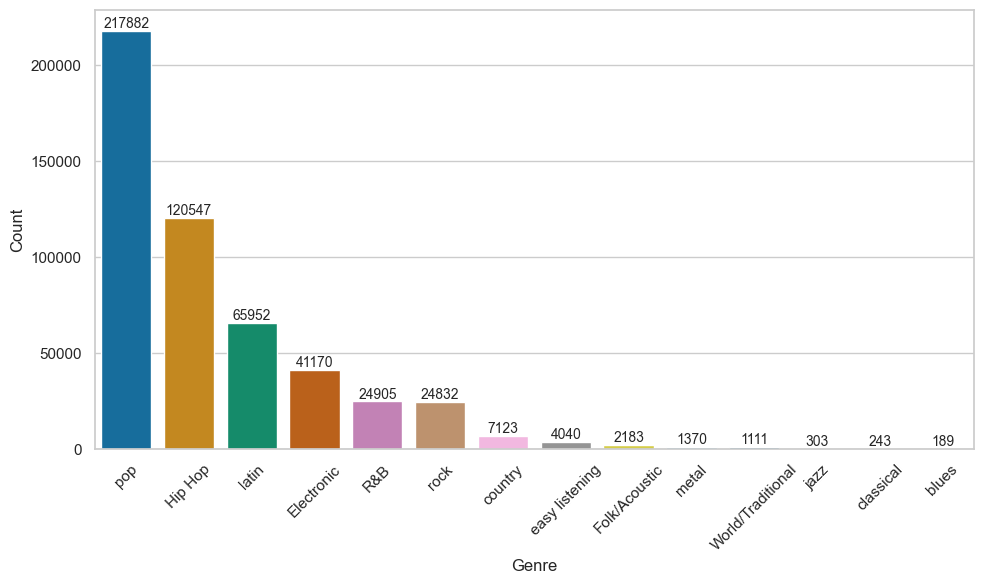
\includegraphics[width=0.8\textwidth]{genre_distribution.png}
    \caption{Distribution of genres in the dataset}
    \label{fig:genre_distribution}
\end{figure}

\section{Confusion matrix for Task 1}
\label{appendix:confusion_matrix}

This confusion matrix displays the result in an intuitive and clear way. Rows (true labels) versus columns (predicted labels) show the correct predictions in its main diagonal. Due to the heave imbalance, most of the instances are concentrated in the \textit{"Pop"} and \textit{"Hip Hop"} classes.

\begin{figure}[h!]
    \centering
    % Adjust the width to reduce the size of the image
    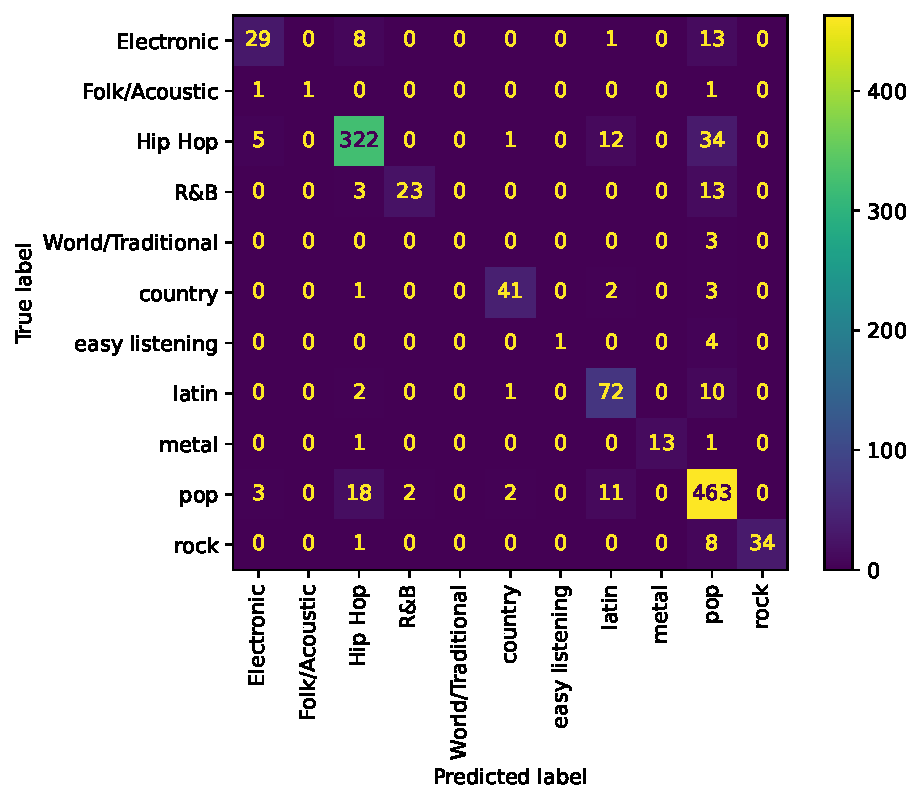
\includegraphics[width=0.7\textwidth]{CatBoost_confusion_matrix.pdf}
    \caption{Confusion matrix obtained on our best model (CatBoost)}
    \label{fig:confusion_matrix}
\end{figure}

\section{Feature importance in Task 1}

To provide further detail into the results of task 1, we provide these images. Two barplots from the best-resulting models (CatBoost and Random Forest) indicate the importance of the features in the models' decision in descending order.

\begin{figure}[h!]
    \centering
    \begin{subfigure}{0.45\textwidth}
        \centering
        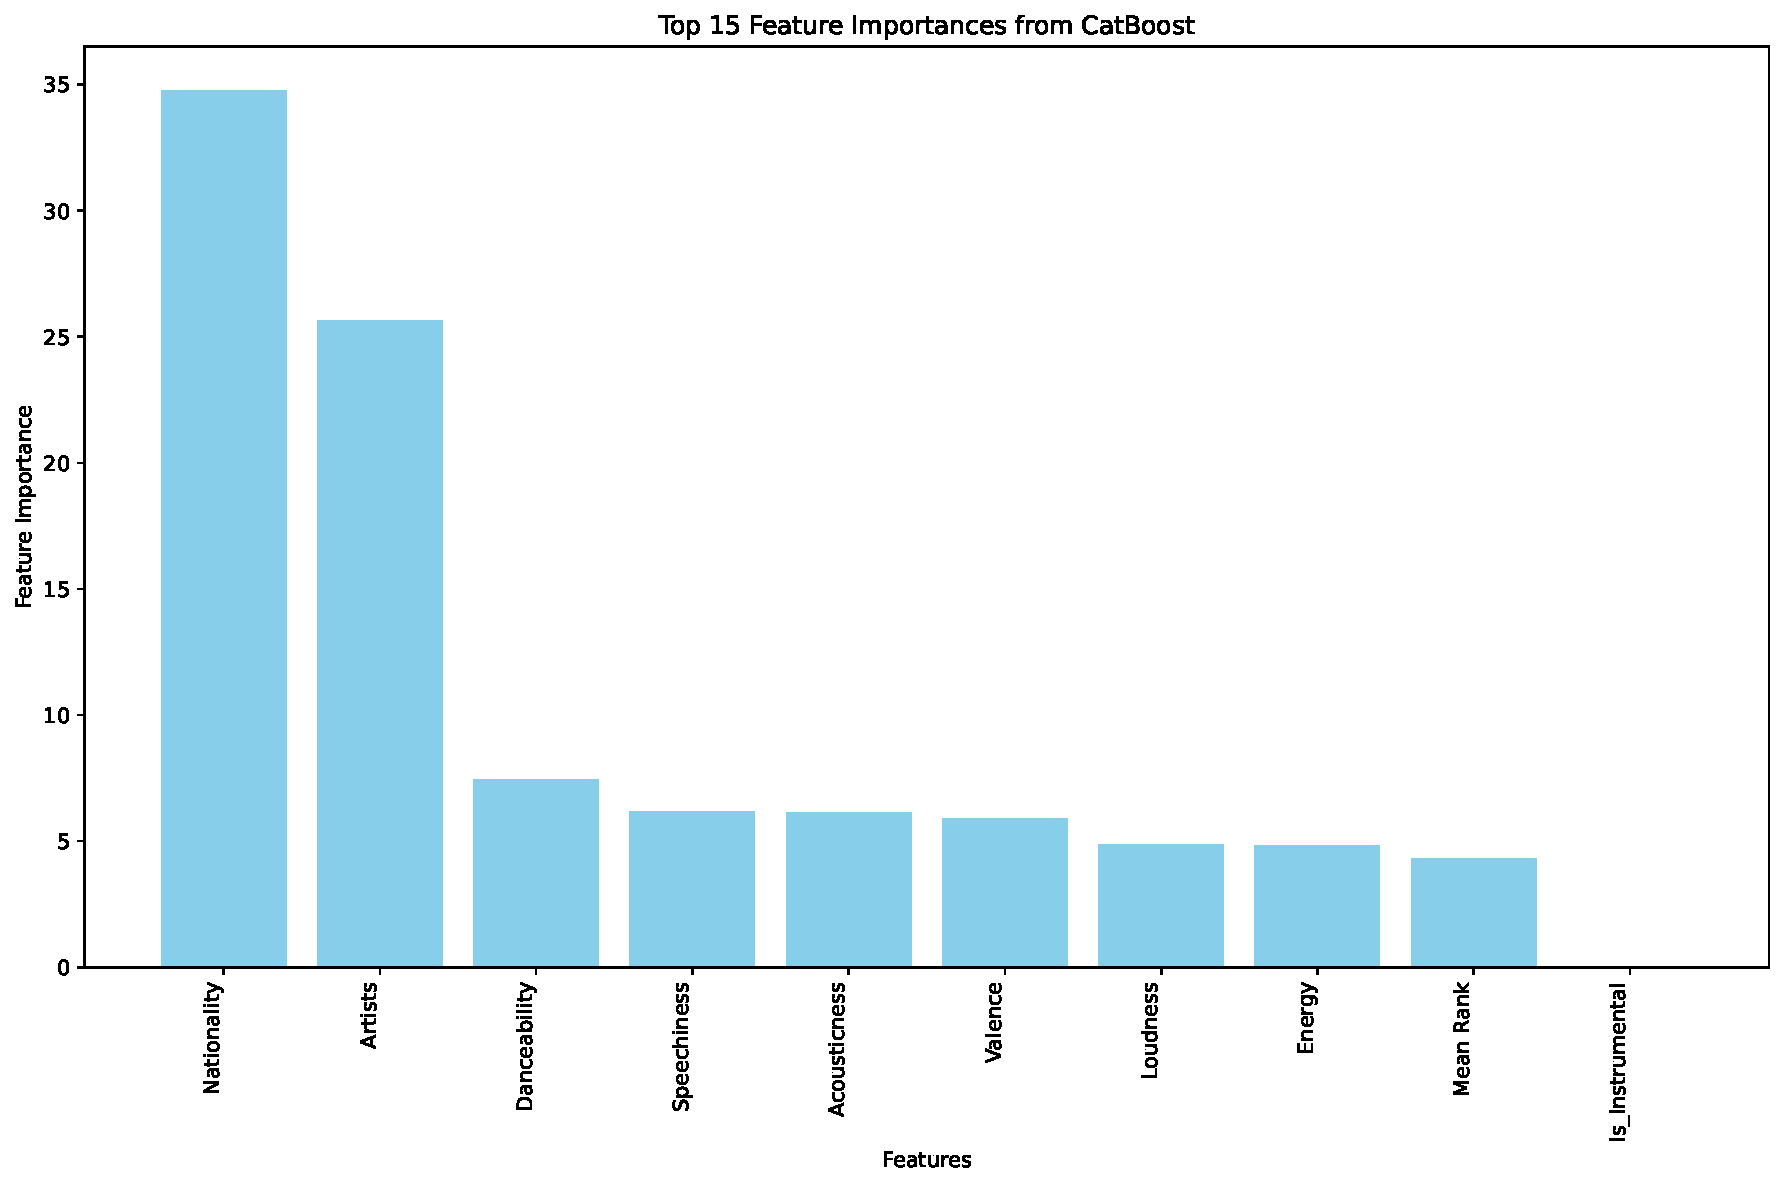
\includegraphics[width=\textwidth]{catboost_importance.pdf}
        \caption{Most important features according to CatBoost}
        \label{fig:subfigure1}
    \end{subfigure}
    \hfill
    \begin{subfigure}{0.45\textwidth}
        \centering
        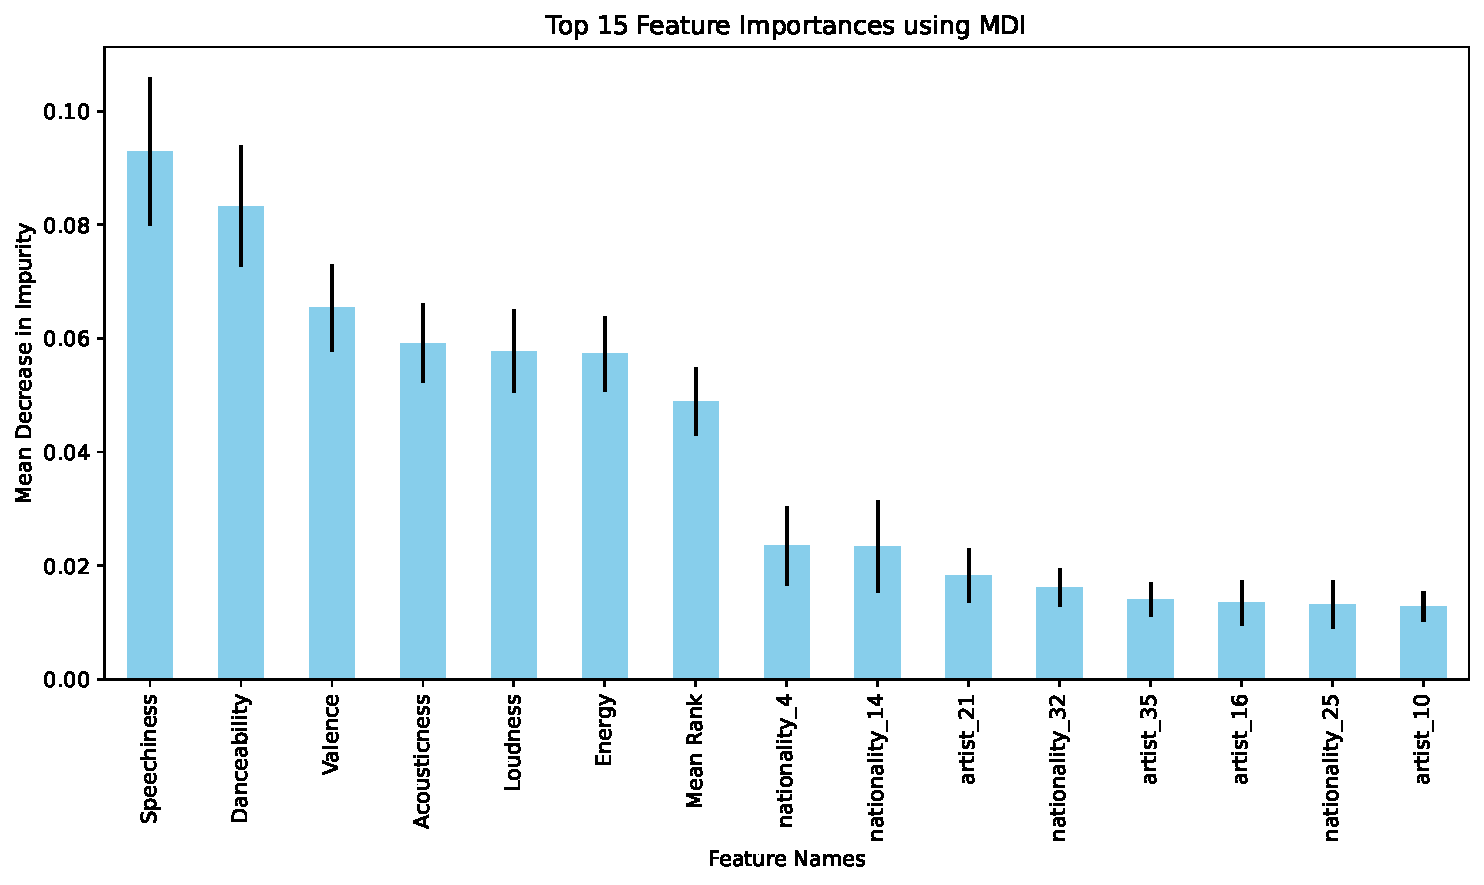
\includegraphics[width=\textwidth]{feature_importance_top15_hash.pdf}
        \caption{Most important features according to Random Forest}
        \label{fig:subfigure2}
    \end{subfigure}
    \caption{Feature importance of our dataset using our 2 of best performing models. Mean Decrease in Impurity (MDI) score is calculated on Random Forest classifier under hash features setting to obtain the results. For CatBoost the average change in the model's prediction when a feature's value is randomly shuffled is measured.}
    \label{fig:feature_importance}
\end{figure}

\section{Hit song prediction}
\label{appendix:hit_song}

The task of hit song prediction involves classifying whether a song became a ``hit'' based on its features. A ``hit'' is defined as a song that at some point achieved a rank higher than 10 on the playlist. The classification task aims to predict this outcome, effectively distinguishing ``hit'' songs from ``not a hit'' songs.

However, the dataset was extremely imbalanced, with the majority of songs classified as ``not a hit'' and very few as ``hit.'' Consequently, all models, including XGBoost, MLP, and Logistic Regression, achieved near-perfect results for the ``not a hit'' class but performed very poorly for the ``hit'' class due to the lack of sufficient training instances.

To address the imbalance, oversampling using SMOTE was applied, generating synthetic samples for the ``hit'' class. Despite this, the models continued to fail to generalize for hits, likely due to the features being insufficient to capture the complexity of what makes a song a hit or the inherent noise in the minority class patterns.

Even with adjustments such as class weights and various resampling strategies, the models overfit to the dominant ``not a hit'' class. Metrics such as accuracy were misleadingly high, as they did not reflect the poor performance on the minority ``hit'' class. Future work could explore data enrichment, advanced resampling methods, or domain-specific models designed for rare-event prediction tasks, but due to time limitations we decided to give a try to different prediction tasks.



\section{Temporal genre prediction}
\label{appendix:temporal_genre_prediction}
We developed a predictive model to forecast the popularity scores of various music genres using the \textit{Points (Total)} and \textit{Date} columns along with additional temporal features. By employing two models—\textbf{Multi-Output Regression with XGBoost} and \textbf{Prophet}—we aimed to compare their effectiveness. Specifically, we evaluated whether capturing interdependencies between genres (as addressed by Multi-Output Regression) offers better predictive performance than modelling individual time-series patterns (as addressed by Prophet).

We used feature engineering to get more temporal features like \textbf{One day Lag} to maintain some continuity and allowing the model to learn from past values, \textbf{7-day Rolling Average} to smooth out short-term fluctuations and highlights long-term trends, and some \textbf{Time-based Features} like Year, month, Quarter, and DayofWeek to help capture the seasonal patterns in genre popularity.

After training both models we were able to forecast the popularity scores of all genres given a specific time and temporal values.

We concluded that \textbf{Prophet} is ideal for genres with strong temporal dynamics, while the \textbf{Multi-Output Regressor} captures inter-genre dependencies and handles irregular patterns. The combined insights from these models provided a comprehensive understanding of genre popularity trends.

\section{Other modelling results}
\label{appendix:other_modelling_results}

\begin{table}[h]
\centering
\begin{tabular}{|c|c|c|c|c|}
\hline
\textbf{Model}      & \textbf{Accuracy} & \textbf{F1-Score (High)} & \textbf{F1-Score (Medium)} & \textbf{F1-Score (Low)} \\ \hline
\textbf{Logistic Regression} & 46\%           & 0.46                     & 0.25                       & \textbf{0.57}          \\ \hline
\textbf{KNN}        & 43\%              & \textbf{0.48}            & 0.32                       & 0.46                   \\ \hline
\textbf{Gaussian Processes Classifier}        & 43\%              & 0.49                     & \textbf{0.13}              & 0.54                   \\ \hline
\end{tabular}
\caption{Comparison of accuracy and F1-scores for each class across the models based on classification reports.}
\label{tab:f1_class_comparison}
\end{table}


\section{Hyperparameter tuning optimal values}
\label{appendix:hyperparameter_tuning}
The following table describes the metrics on validation data for the best models after hyperparameter tuning on \textbf{XGBoost}, \textbf{SVC} \& \textbf{Random Forest}.
\begin{table}[h]
\centering
\begin{tabular}{|c|c|c|c|c|}
\hline
\textbf{Model}      & \textbf{Accuracy} & \textbf{F1-Score (High)} & \textbf{F1-Score (Medium)} & \textbf{F1-Score (Low)} \\ \hline
\textbf{XGBoost}    & 53\%              & 0.53                     & 0.49                       & 0.57                   \\ \hline
\multicolumn{5}{|l|}{\textit{\footnotesize{Hyperparameters: colsample\_bytree=0.8, gamma=1, learning\_rate=0.01, max\_depth=7,}}} \\ 
\multicolumn{5}{|l|}{\textit{\footnotesize{n\_estimators=200, scale\_pos\_weight=1, subsample=0.8}}} \\ \hline
\textbf{SVC}        & 44\%              & 0.42                     & 0.13                       & 0.56                   \\ \hline
\multicolumn{5}{|l|}{\textit{\footnotesize{Hyperparameters: C=1, class\_weight=\{0: 1.0, 1: 1.0, 2: 1.0\}, gamma=1, kernel=rbf}}} \\ \hline
\textbf{Random Forest} & \textbf{54\%}  & \textbf{0.54}            & \textbf{0.52}              & \textbf{0.56}          \\ \hline
\multicolumn{5}{|l|}{\textit{\footnotesize{Hyperparameters: class\_weight=balanced, max\_depth=20, max\_features=sqrt,}}} \\
\multicolumn{5}{|l|}{\textit{\footnotesize{min\_samples\_leaf=2, min\_samples\_split=5, n\_estimators=300}}} \\ \hline
\end{tabular}
\caption{Comparison of accuracy and F1-scores for each class across the models after hyperparameter tuning in task 2.}
\label{tab:f1_class_comparison_tuned}
\end{table}

The hyperparameters selected for tuning were chosen based on their direct impact on model performance and ability to capture complex patterns in the data:

\begin{itemize}
    \item \textbf{Random Forest:}
    \begin{itemize}
        \item \texttt{max\_depth}: Controls tree complexity to avoid overfitting.
        \item \texttt{max\_features}: Optimizes the number of features used for splits to improve efficiency and performance.
        \item \texttt{min\_samples\_leaf, min\_samples\_split}: Ensure meaningful splits, reducing over-splitting.
        \item \texttt{n\_estimators}: Determines the number of trees, balancing accuracy and computational cost.
        \item \texttt{Optimal values for task 1:} 'None', 'sqrt', 1, 200
    \end{itemize}

    \item \textbf{XGBoost:}
    \begin{itemize}
        \item \texttt{colsample\_bytree, subsample}: Improve tree diversity by limiting features and samples used per tree.
        \item \texttt{gamma}: Penalizes overly complex splits to improve generalization.
        \item \texttt{learning\_rate}: Allows gradual convergence for more accurate predictions.
        \item \texttt{max\_depth}: Balances tree complexity with performance.
        \item \texttt{n\_estimators}: Controls the number of boosting rounds for optimal performance.
    \end{itemize}

    \item \textbf{SVC:}
    \begin{itemize}
        \item \texttt{C}: Balances the trade-off between misclassification and margin size.
        \item \texttt{gamma}: Adjusts the influence of training samples on the decision boundary.
        \item \texttt{kernel}: The RBF kernel was selected for its flexibility in modelling non-linear patterns.
    \end{itemize}

    \item \textbf{Logistic Regression:}
    \begin{itemize}
        \item \texttt{penalty}: Specifies the type of regularization to use (e.g., \texttt{l2} for Ridge regularization), which helps prevent overfitting by penalizing large coefficients.
        \item \texttt{C}: Controls the inverse strength of regularization. Smaller values imply stronger regularization, encouraging simpler models.
        \item \texttt{solver}: Defines the optimization algorithm to use for training (e.g., \texttt{lbfgs}, \texttt{saga}), which affects computational efficiency and compatibility with the dataset size.
        \item \texttt{max\_iter}: Sets the maximum number of iterations the solver will run, ensuring convergence for larger or more complex datasets.
        \item \texttt{Optimal values for task 1:} 'L2', 10, 'newton-cg', 100
    \end{itemize}

    \item \textbf{Gradient Boosting:}
    \begin{itemize}
        \item \texttt{n\_estimators}: Specifies the number of boosting iterations (trees). Higher values improve performance but may increase training time and risk overfitting.
        \item \texttt{learning\_rate}: Controls the contribution of each tree to the overall model. Smaller values require more trees but improve generalization.
        \item \texttt{max\_depth}: Limits the maximum depth of each tree, balancing model complexity with performance by preventing overly deep trees.
        \item \texttt{min\_samples\_split}: Defines the minimum number of samples required to split a node, influencing tree growth and preventing overfitting.
        \item \texttt{min\_samples\_leaf}: Specifies the minimum number of samples required to be at a leaf node, helping regularize the tree by limiting leaf sizes.
        \item \texttt{Optimal values for task 1:} 200, 0.1, 4, 5, 2
    \end{itemize}

    \item \textbf{CatBoost:}
    \begin{itemize}
        \item \texttt{iterations}: Specifies the number of boosting iterations (trees). Higher values allow the model to learn more complex patterns but increase training time and risk of overfitting.
        \item \texttt{learning\_rate}: Determines the contribution of each tree to the final model. Smaller values lead to slower convergence but can improve generalization.
        \item \texttt{depth}: Controls the maximum depth of each tree, balancing model complexity and performance. Deeper trees can capture more intricate relationships but may overfit.
        \item \texttt{Optimal values for task 1:} 200, 0.1, 6
    \end{itemize}


\end{itemize}

Other hyperparameters, such as \texttt{criterion} in Random Forest or \texttt{shrinking} in SVC, were not tuned as they have minimal impact on predictive performance or primarily affect computational efficiency.

\newpage
\section{PCA for for Task 2}
\label{appendix:pca_non_linear_data}

Dimensionality reduction in 3 and 2 dimensions is used to visualize the dataset. Though in the 2D example no apparent linear separabilty is observed, the 3D plot seems to exhibit a cluster for the \textit{Low} class, though it still does not explicitly show signs of clear separabilty.

\begin{figure}[h]
    \centering
    \begin{subfigure}[b]{0.45\textwidth}
        \centering
        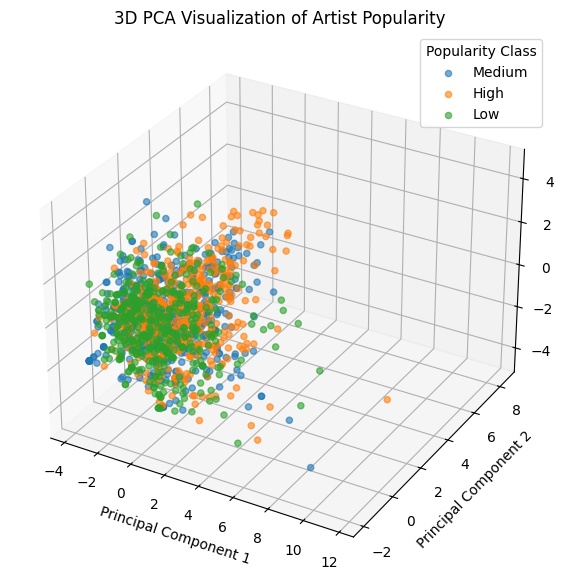
\includegraphics[width=\textwidth]{pca2d_task2.png}
        \caption{2D PCA Visualization}
        \label{fig:pca2d}
    \end{subfigure}
    \hfill
    \begin{subfigure}[b]{0.45\textwidth}
        \centering
        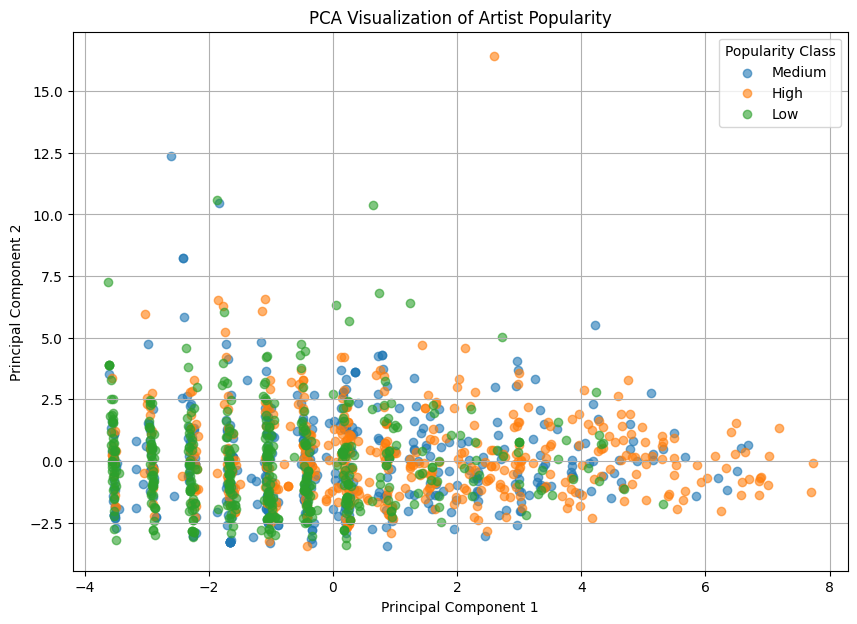
\includegraphics[width=\textwidth]{pca3d_task2.png}
        \caption{3D PCA Visualization}
        \label{fig:pca3d}
    \end{subfigure}
    \caption{PCA Visualizations for Task 2 in 2D and 3D.}
    \label{fig:pca_task2}
\end{figure}

We can clearly observe non-linear separable data and that is why using models that are capable of doing this kind of separations were chosen.

\section{Team member contribution}
Our team collaborated effectively to analyse the dataset and produce this report. Initially, each member conducted separate Exploratory Data Analysis (EDA), providing unique insights. We then discussed and combined these individual efforts into a unified EDA task, which is detailed in the report. Based on our combined insights, we identified key questions to explore as a team. Each member selected one question and independently built models to address it. After obtaining results, we collectively decided on the two main tasks to include in the report, aligning with the assignment requirements and our consensus. Additional tasks we worked on are documented in the appendix, as they couldn't be included in the main report due to space constraints. Finally, all team members contributed to writing and formatting the report, ensuring a cohesive and well-structured presentation.

\end{document}

%%% Local Variables:
%%% mode: latex
%%% TeX-master: t
%%% End:
